\documentclass{IEEEcsmag}

\usepackage[colorlinks,urlcolor=blue,linkcolor=blue,citecolor=blue]{hyperref}
\expandafter\def\expandafter\UrlBreaks\expandafter{\UrlBreaks\do\/\do\*\do\-\do\~\do\'\do\"\do\-}
\usepackage{upmath,color}


\jvol{XX}
\jnum{XX}
\paper{8}
\jmonth{Month}
\jname{Publication Name}
\jtitle{Publication Title}
\pubyear{2021}

\newtheorem{theorem}{Theorem}
\newtheorem{lemma}{Lemma}


\setcounter{secnumdepth}{0}

\begin{document}

\sptitle{Article Type: Description  (see below for more detail)}

\title{Title: No More Than Four Lines}

\author{First A. Author}
\affil{University of California, Berkeley, CA, 94720, USA}

\author{Second Author Jr.}
\affil{Company, City, (State), Postal Code, Country}

\author{Third Author III}
\affil{Institute, City, (State), Postal Code, Country}

\markboth{THEME/FEATURE/DEPARTMENT}{THEME/FEATURE/DEPARTMENT}

\begin{abstract}\looseness-1Abstract text goes here. To find your publication's abstract\break word count limit, navigate to your magazine's homepage from\break \href{https://www.computer.org/csdl/magazines}{https://www.computer.org/csdl/magazines} and click Write for Us $>$Author Information. An abstract is a single paragraph that summarizes the significant aspects of the manuscript. Often it indicates whether the manuscript is a report of new work, a review or overview, or a combination thereof. Do not cite references in the abstract. Papers must not have been published previously and must be targeted toward the general technical reader. Papers submitted for peer review (not departments or columns) may fit into the theme of an open Call for Papers or be submitted as a ``Regular'' paper. Some Computer Society (CS) magazines provide early access to full manuscript submissions by posting a preprint of the article prior to its inclusion in an issue. Preprint articles are considered published and may be cited using their Digital Object Identifier (DOI). IEEE's Publishing Operations team will provide editorial and production services throughout the publication process.
\end{abstract}

\maketitle


\chapteri{T}he introduction should provide background information (including relevant references) and should indicate the purpose of the manuscript. Cite relevant work by others, including research outside your company or institution. Place your work in perspective by referring to other research\break papers.


This document is a template for file type LaTeX. If you are reading a paper or PDF version of this document, please download the electronic file, CsMag template.tex, from the IEEE Template Selector at \href{https://template-selector.ieee.org}{template-selector.ieee.org} so you can use it to prepare your manuscript. Articles that are math heavy are encouraged to use the LaTeX version of the\break  template.


In the header at the top of page 1, please indicate whether your article is a Theme Article, Feature Article, or Department submission. If it is a Theme Article, include the special issue title as the description. If it is a Feature Article, please provide a 3-4 word phrase reflecting the topic of the article. If it is a Department submission, please name the\break department.\vadjust{\pagebreak} 

\section{COPYRIGHT AND OPEN ACCESS}

Upon acceptance, all CS magazine corresponding authors must complete IEEE's Electronic Copyright Form (eCF), which will be prompted at the start of the production process. Further details about IEEE's copyright policies are available at \href{https://www.ieee.org/publications/rights/index.html}{www.ieee.org/publications/rights/index.html}. 

CS magazines now offer an open access model for full-length research articles. At the time of submission to the ScholarOne peer review portal, authors will have the option to indicate that they will pay for open access. Should the article be accepted, authors will receive information on how to proceed with payment and licensing. More information on the hybrid open access program for magazines can be found at \href{https://open.ieee.org/index.php/about-ieee-open-access/faqs}{open.ieee.org/index.php/about-ieee-open-access/faqs}.\vspace*{-10pt}


\section{FONTS}

This template utilizes Adelle Sans for body text and and Computer Modern for math.\vspace*{-5pt}

\begin{figure}
\centerline{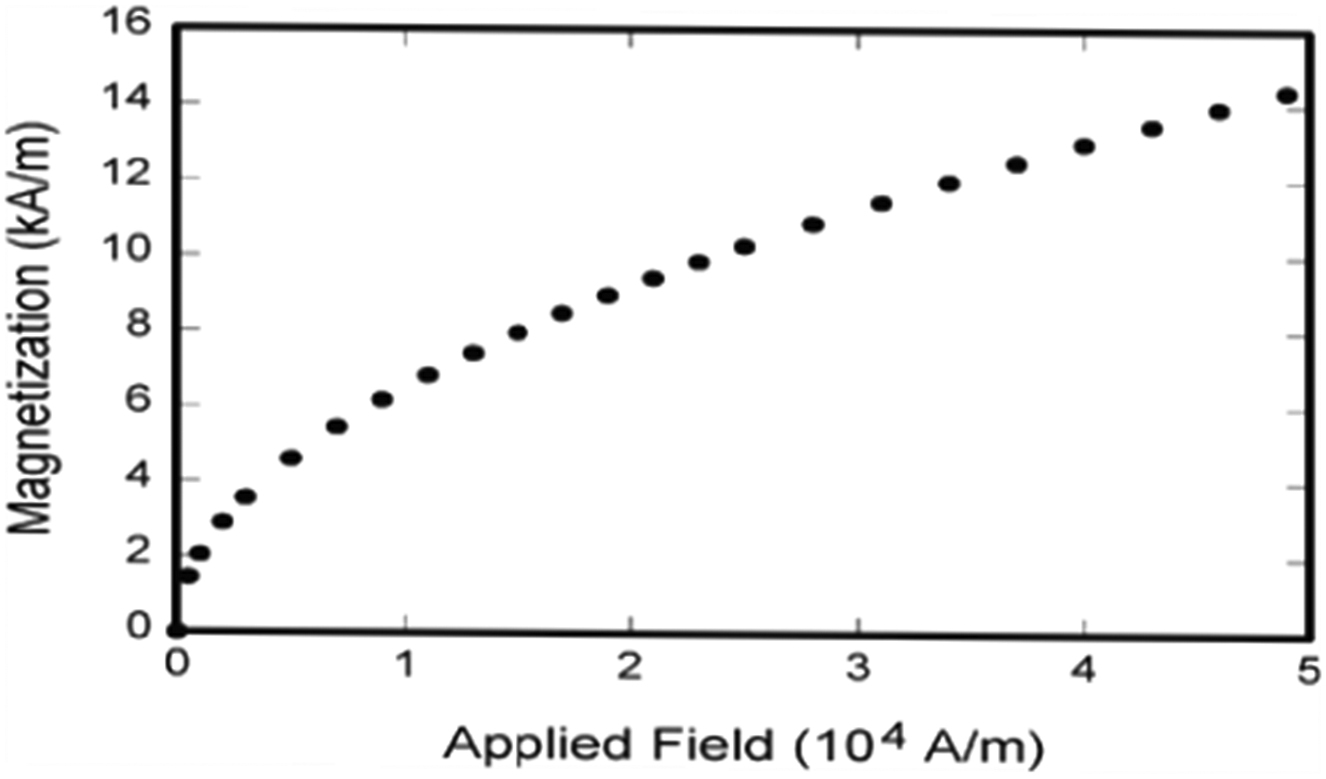
\includegraphics[width=18.5pc]{fig1.jpg}}
\caption{Note that ``Figure'' is spelled out. There is a period after the figure number, followed by one space. It is good practice to briefly explain the significance of the figure in the caption. (From [``Title''],$^1$ used with permission.)}\vspace*{-5pt}
\end{figure}


\section{SECTIONS}


Sections following the introduction should present results and findings. To find your\vadjust{\pagebreak} publication's word count requirements and limits, navigate to your magazine's homepage from \href{https://www.computer.org/csdl/magazines}{www.computer.org/csdl/magazines}, then click Write for Us $>$Author Information. The manuscript should be written so that each sentence, equation, figure, and table flow smoothly and logically. Relevant work by others, as well as relevant products from other companies, should be adequately and accurately cited (see the Reference Style section). Sufficient support should be provided (or cited) for the assertions made and conclusions drawn.

Headings are unnumbered with no ending punctuation.\vspace*{-5pt} 



\section{MAGAZINE STYLE}
Use American English when writing the paper. The serial comma should be used (``a, b, and c'' not ``a, b and c''), and periods and commas appear within quotation marks, like ``this period.'' Other punctuation is placed ``outside''! Avoid the use of technical jargon, slang, and vague or informal English. Generic technical terms should instead be used, as magazine articles are meant to be understandable by a broad readership.\vspace*{-5pt}



\subsection{Acronyms and Abbreviations}

\looseness-1All acronyms should be defined at first mention in the abstract and in the main text. Define in figures and tables only if not defined in the discussion of the figure/table. Acronyms consist of capital letters (except where salted with lowercase), but the terms they represent need not be given initial caps unless a proper name is involved [``central processing unit'' (CPU) but ``Fourier transform'' (FT)]. Use of ``e.g.'' and ``i.e.'' is okay in parenthetical statements, but avoid using ``etc.''


Abbreviate units of time (s, min, hr, mo, yr) only in virgule constructions (10 $\umu$g/hr) and in artwork; otherwise, spell out (e.g., 3 months, 25 minutes). Units of measure (such as Kb, MB, kWh) should always be abbreviated when used with a numeral; if used alone, spell out (``16 MB of RAM'' but ``these values are measured in micrometers'').


\begin{table}
\vspace*{4pt}
\caption{Units for magnetic properties.}
\label{table}
\tablefont
\begin{tabular*}{17.5pc}{@{}p{29pt}p{63pt}<{\raggedright}p{80pt}<{\raggedright}@{}}
\toprule
Symbol& 
Quantity& 
Conversion from Gaussian and  CGS EMU to SI$^{\mathrm{a}}$ \\
\colrule
$\Phi $& 
Magnetic flux& 
1 Mx $\to  10^{-8}$ Wb $= 10^{-8}$ V $\cdot$ s \\[3pt]
$B$& 
Magnetic flux density,   magnetic induction& 
1 G $\to  10^{-4}$ T $= 10^{-4}$ Wb/m$^{2}$ \\[3pt]
$H$& 
Magnetic field strength& 
1 Oe $\to  10^{-3}/(4\pi )$ A/m \\[3pt]
$m$& 
Magnetic moment& 
1 erg/G $=$ 1 emu   $\to 10^{-3}$ A $\cdot$ m$^{2} = 10^{-3}$ J/T \\[3pt]
$M$& 
Magnetization& 
1 erg/(G $\cdot$ cm$^{3}) =$ 1 emu/cm$^{3}$   $\to 10^{-3}$ A/m \\[3pt]
4$\pi M$& 
Magnetization& 
1 G $\to  10^{-3}/(4\pi )$ A/m \\
\botrule
\multicolumn{3}{@{}p{17.5pc}@{}}{$^{{\rm a}}$Gaussian units are the same as cg emu for magnetostatics; Mx 
$=$ maxwell, G $=$ gauss, Oe $=$ oersted; Wb $=$ weber, V $=$ volt, s $=$ 
second, T $=$ tesla, m $=$ meter, A $=$ ampere, J $=$ joule, kg $=$ 
kilogram, H $=$ henry.}
\end{tabular*}\vspace*{8pt}
\label{tab1}
\end{table}


\subsection{Numbers}

Spell out numerals up to ten that have no unit of measure or time (one, two  ten), but always use numerals with units of time and measure. Some examples are as follows: 11 through 999; 1000; 10,000; 20th century; twofold, tenfold, 20-fold; two times; 0.2~cm; $p=.001$; 25\%; 10\% to 25\%.


\section{MATH AND EQUATIONS}

Use either the Microsoft Equation Editor or the MathType plugin, which can be obtained from https://store.wiris.com/en/products/mathtype/download. For help with formatting and placing equations, refer to the IEEE Editing Math Guide at \url{http://journals.ieeeauthorcenter.ieee.org/wp-content/uploads/sites/7/Editing-Mathematics.pdf} and the IEEE MathType Tutorial for Microsoft Word Users at \url{http://journals.ieeeauthorcenter.ieee.org/wp-content/uploads/sites/7/IEEE-Math-Typesetting-Guide-for-MS-Word-Users.pdf}.


Scalar {\it variables} and {\it physical constants} should be italicized, and a bold (non-italics) font should be used for {\bf vectors} and {\bf matrices}. Do not italicize subscripts unless they are variables.

Equations should be either display (with a number in parentheses) or inline.   

If a display equation cannot be centered, the first line can be made flush left to the column to allow more room for the following lines of the equation.


Be sure the symbols in your equation have been defined before the equation appears or immediately following. Please refer to ``(1),'' not ``Eq. (1)'' or ``equation (1).''

Punctuate display equations when they are part of the sentence preceding it, as in
\begin{equation}
A=\pi r^2
\end{equation}

If the text following the equation flows logically as a part of the display equation, such as
\begin{equation}
a^2 + b^2 = c^2, 
\end{equation}
treat the display equation as you would inline text, using punctuation after the equation as necessary.\vspace*{3.5pt}

\section{LISTS}

If you use a list, keep it short:

\begin{itemize}
\item[{\ieeeguilsinglright}] {\it Style for bulleted lists}---This is the style that should be used for bulleted lists.
	
\item[{\ieeeguilsinglright}] {\it Punctuation in lists}---Each item in the list should end with a period, regardless of whether full sentences are used.

\item[{\ieeeguilsinglright}] {\it Style for numbered lists}---Use 1), 2), 3) followed by a), b), c), and then i), ii), iii).

\end{itemize}\vspace*{3pt}




\begin{figure*}
\centerline{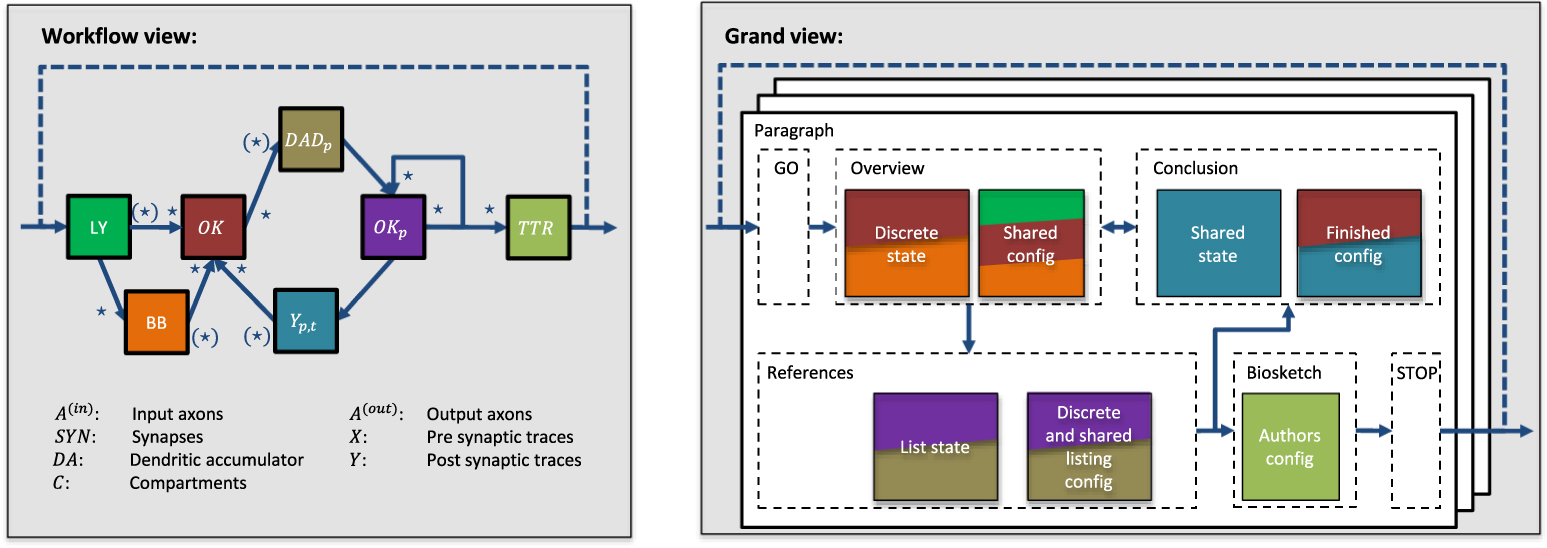
\includegraphics[width=26pc]{fig2.jpg}}
\caption{Note that ``Figure'' is spelled out. There is a period after the figure number, followed by one space. It is good practice to briefly explain the significance of the figure in the caption. (From [``Title''],$^2$ used with permission.)}\vspace*{-5pt}
\end{figure*}




\section{FIGURES AND TABLES}

\subsection{In-Text Callouts for Figures and Tables}

Figures and tables must be cited in the running text in consecutive order. Figure callouts should be Roman, not bold or italic, like this: ``see Figure 1.'' Figure 2 shows an example of a figure spanning two columns.

Vertical lines are optional in tables. Footnotes should be indicated by a, b, c, d, and so on, per the \emph{Chicago Manual of Style} (see Table 1). Statements that serve as captions for the entire table do not need footnote letters. 

Authors are responsible for obtaining permission to reprint previously published figures or tables. Required permission information should be included in the figure/table caption, for instance: ``From `[Title],'$^1$ with permission,'' or ``Adapted from `[Title],'$^2$ with permission.'' \emph{Carefully} explain each figure in the text. To find your publication's figure limit, if applicable, navigate to your magazine's homepage from \href{https://www.computer.org/csdl/magazines}{www.computer.org/csdl/magazines} and click Write for Us $>$ Author Information.




\section{REFERENCE STYLE}
References must be cited in text. They appear as superscript outside the punctuation, and are listed in the References section in the order that they appear in text. Do not refer to the reference number or use ``Ref.'' or ``reference'' in text. Instead of writing ``References~3--5 show$\ldots$,'' construct the sentence independently of its reference callout; for example, ``The XYZ study shows$\ldots$.''$^{3-5}$ Please do not use automatic endnotes in Word; rather, type the reference list at the end of the paper using the ``References'' style.

Reference numbers are set flush left and form a column of their own, hanging out beyond the body of the reference. The reference numbers are on the line and end with period. In all references, the given name of the author or editor is abbreviated to the initial(s) only and precedes the last name. Include all names; use \emph{et al}. only if names are more then six. Do not use commas around Jr., Sr., and III in names. Abbreviate conference titles. When citing IEEE magazines or transactions, provide the issue number, page range, volume number, year, and/or month if available. When referencing a patent, provide the day and the month of issue or application. Please obtain and include relevant reference information. Do not combine references. There must be only one reference with each number. If there is a URL included with the print reference, it can be included at the end of the reference. When citing a preprint, please include the Digital Object Identifier (DOI).

Other than books, capitalize only the first word in a paper title, except for proper nouns and element symbols. For papers published in translation journals, please give the English citation first, followed by the original foreign-language citation. See the end of this document for formats and examples of common references.\vspace*{4pt}

\section{APPENDIX SECTION}

 The Appendix is moved to supplementary material if it is not discussed/referenced in the main text. If it is discussed in the text, it is set as a sidebar.  


\section{SUPPLEMENTARY MATERIAL}

If supplementary material is provided in the article, then it is deleted. A pointer to the supplemental material will be added to the first callout in the article and the phrase “available online” will be added to all subsequent callouts.

\subsection{Examples:}
\subsubsection{First Callout:} 

See the Appendix, which is available in the IEEE Computer Society Digital Library at \url{http://doi.ieeecomputersociety.org/10.1109/MCSE.2019.2947017}.

For detailed algorithms, please refer to the supplementary materials, which can be found in the Computer Society Digital Library at \url{http://doi.ieeecomputersociety.org/10.1109/MCSE.2019.2947017}.\vspace*{-8pt}

\subsubsection{Second Callout:}

More experimental results are presented in the supplementary materials, available online, due to the space limitation.\vspace*{-8pt}


\section{CONCLUSION}
The manuscript should include future directions of the research. Authors are strongly encouraged not to reference multiple figures or tables in the conclusion; these should be referenced in the body of the paper.\vspace*{-8pt}


\section{ACKNOWLEDGMENTS}
The Acknowledgments is always plural even if there is a single acknowledgment. The author(s) would like to thank A, B, and C. This work was supported by XYZ under Grant \#\#\#.


The ``Acknowledgments'' (spelled with just two e's, per American English) section appears immediately after the conclusion and before the reference list. Sponsor and financial support  are included in the acknowledgments section. For example: ``This work was supported in part by the U.S. Department of Commerce under Grant 123456.'' If support for a specific author is given, then use the following example for correct  wording. ``The work of First A. Author was supported by the U.S. Department of Commerce under Grant 123456''. Researchers that contributed information or assistance to the article should also be acknowledged in this section, and expressions should be simple and expressed as ``We thank$\ldots$,'' rather than indicating which of the authors is doing the thanking. Also, if corresponding authorship is noted in the paper, it should be placed in the bio of the corresponding author.


\def\refname{REFERENCES}

\begin{thebibliography}{1}

\bibitem{AA1}
G. M. Amdahl, G. A. Blaauw, and F. P. Brooks, ``Architecture of the IBM System/360,'' {\it IBM J. Res. Dev}., vol. 8, no. 2, pp. 87--101, 1964. (Journal)

\bibitem{BB1}
IBM Corporation, IBM Knowledge Center - IBM Secure Service Container (Secure Service Container). [Online]. Available: {https://www.ibm.com/support/\break knowledgecenter/en/HW11R/com.ibm.hwmca.kc\_se.doc/\break introductiontotheconsole/wn2131zaci.html} (URL)

\bibitem{CC1}
J. Williams, ``Narrow-band analyzer,'' Ph.D. dissertation, Dept.  Elect. Eng., Harvard Univ., Cambridge, MA, USA, 1993. (Thesis or dissertation)

\bibitem{DD1}
J. M. P\'erez, R. Berlanga, M. J. Aramburu, and T. B. Pedersen, ``Integrating data warehouses with web data: A survey,'' {\it IEEE Trans. Knowl. Data Eng}., early access, Dec. 21, 2007, doi:10.1109/TKDE.2007.190746. (Preprint)

\bibitem{EE1}
W.-K. Chen, {\it Linear Networks and Systems}. Belmont, CA, USA: Wadsworth,  1993, pp. 123--135. (Book)

\bibitem{FF1}
S. P. Bingulac, ``On the compatibility of adaptive controllers,'' in {\it Proc. 4th Ann. Allerton Conf. Circuits Syst. Theory}, 1994,  pp. 8--16. (Conference proceedings)

\bibitem{GG1}
K. Elissa, ``An overview of decision theory,'' unpublished. (Unpublished manuscript)

\bibitem{HH1}
R. Nicole, ``The last word on decision theory,'' {\it J. Comput. Vis.}, submitted for publication. (Pending publication)

\bibitem{II1}
C. J. Smith and J. S. Smith, Rocky Mountain Research Laboratories, Boulder, CO, USA, private communication, 1992. (Private communication)
\end{thebibliography}\vspace*{-8pt}


\begin{IEEEbiography}{First A. Author}{\,}All biographies are limited to one paragraph, following the structure given here. For features, provide each author's current role and institution (to match the first page of the article); three very brief current research interests; highest degree, topic, and awarding institution (do not include year); professional memberships, such as the IEEE Computer Society and any grade information; and contact information in the form of an email address. For departments, provide each author's current role, institution, and contact information in the form of an email address. Examples are below. \vadjust{\vfill\pagebreak}
\end{IEEEbiography}

\begin{IEEEbiography}{Second B. Author Jr.}{\,} is a researcher at the  ABC Corporation, B\"oblingen, Germany.  Her current research interests include a, b, and c. Author received her Ph.D. degree  in physics from University. She is a Fellow of the IEEE Computer Society. Contact her at sbauthor@abc.com.\vspace*{8pt}
\end{IEEEbiography}

\begin{IEEEbiography}{Third C. Author III} {\,} is a program officer at the  DEF Corporation, Tokyo, Japan. Contact him at tcauthor@def.com.
\end{IEEEbiography}

\end{document}

